\input{preambulo_presentacion_Berlin_beaver}
\usepackage{pifont}
\usepackage{siunitx}
\usetikzlibrary{shapes}
\newcommand{\cmark}{\ding{51}}%
\newcommand{\xmark}{\ding{55}}%
\definecolor{cadmiumgreen}{rgb}{0.0, 0.42, 0.24}
\makeatletter
\setbeamertemplate{footline}
{
  \leavevmode%
  \hbox{%
  \begin{beamercolorbox}[wd=.333333\paperwidth,ht=2.25ex,dp=1ex,center]{section in foot}%
    \usebeamerfont{section in foot} \insertsection
  \end{beamercolorbox}%
  \begin{beamercolorbox}[wd=.333333\paperwidth,ht=2.25ex,dp=1ex,center]{subsection in foot}%
    \usebeamerfont{subsection in foot}  \insertsubsection
  \end{beamercolorbox}%
  \begin{beamercolorbox}[wd=.333333\paperwidth,ht=2.25ex,dp=1ex,right]{date in head/foot}%
    \usebeamerfont{date in head/foot} \insertshortdate{} \hspace*{2em}
    \insertframenumber{} / \inserttotalframenumber \hspace*{2ex} 
  \end{beamercolorbox}}%
  \vskip0pt%
}
\makeatother
%--------------------------------------------------------------------
%--------------------------------------------------------------------
\newcounter{choice}
\renewcommand\thechoice{\Alph{choice})}
%\newcommand\choicelabel{\thechoice.}
\newcommand\choicelabel{\thechoice}

\newenvironment{choices}%
  {\list{\choicelabel}%
     {\usecounter{choice}\def\makelabel##1{\hss\llap{##1}}%
       \settowidth{\leftmargin}{W.\hskip\labelsep\hskip 2.5em}%
       \def\choice{%
         \item
       } % choice
       \labelwidth\leftmargin\advance\labelwidth-\labelsep
       \topsep=0pt
       \partopsep=0pt
     }%
  }%
  {\endlist}

\newenvironment{oneparchoices}%
  {%
    \setcounter{choice}{0}%
    \def\choice{%
      \refstepcounter{choice}%
      \ifnum\value{choice}>1\relax
        \penalty -50\hskip 1em plus 1em\relax
      \fi
      \choicelabel
      \nobreak\enskip
    }% choice
    % If we're continuing the paragraph containing the question,
    % then leave a bit of space before the first choice:
    \ifvmode\else\enskip\fi
    \ignorespaces
  }%
  {}
%----------------------------------------------------------
%----------------------------------------------------------

\setbeamertemplate{navigation symbols}{}
\date{19 de marzo de 2021}
\title{Sesión 4. Razonamiento matemático}
\subtitle{Asesoría}
\begin{document}
\maketitle
\fontsize{14}{14}\selectfont
\spanishdecimal{.}
\section*{Contenido}
\frame[allowframebreaks]{\tableofcontents[currentsection, hideallsubsections]}
\section{Habilidad matemática}
\frame{\tableofcontents[currentsection, hideothersubsections]}

\subsection{Batería de ejercicios}

\begin{frame}
\frametitle{Ejercicio 1}
La suma de $2$ números es $12$ y su diferencia $6$, ¿cuáles son esos números?
\begin{choices}
\choice $7,\, 5$
\choice $8, \, 4$ \\
\choice $10, \, 2$ \\
\choice $9, \, 3$ \\
\choice $11, \, 1$ \\
\end{choices}
% \pause
% \begin{tikzpicture}[overlay]
%     \node [text = cadmiumgreen] at (1, 1.7) {\cmark};
% \end{tikzpicture}
\end{frame}
\begin{frame}
\frametitle{Otro tipo de ejercicio}
Este ejercicio plantea dos premisas en el enunciado:
\setbeamercolor{item projected}{bg=blue!70!black,fg=yellow}
\setbeamertemplate{enumerate items}[circle]
\begin{enumerate}[<+->]
\item La suma de $2$ números es $12$.
\item Y su diferencia es $6$.
\end{enumerate}
\pause
Entonces tendremos que plantear de alguna manera la información que nos están dando.
\\
\bigskip
\pause
Tendremos que apoyarnos con el \emph{álgebra}.
\end{frame}
\begin{frame}
\frametitle{La primera premisa}
Llamemos a los dos números como $a$ y $b$.
\pause
Entonces la primera premisa nos dice: \enquote{La suma de $2$ números es $12$}.
\pause
Que expresamos como:
\begin{align*}
a + b =  12
\end{align*}
\end{frame}
\begin{frame}
\frametitle{la segunda premisa}
Como ya hemos nombrado a los dos números como $a$ y $b$, expresamos la segunda premisa: \enquote{y su diferencia es $6$}. Quedando como:
\begin{align*}
a - b =  6
\end{align*}
\pause
El siguiente paso es juntar las dos premisas.
\end{frame}
\begin{frame}
\frametitle{Sistema de ecuaciones}
Tenemos entonces un sistema de dos ecuaciones que involucran a los dos números:
\begin{align*}
a + b &= 12 \\[0.5em]
a - b &= 6
\end{align*}
Es un sistema de dos ecuaciones con dos incógnitas.
\end{frame}
\begin{frame}
\frametitle{Solución al sistema simultáneo}
Este sistema simultáneo se resuelve de la siguiente manera: consideramos una incógnita ya sea $a$ o $b$, para encontrar un valor.
\\
\bigskip
\pause
Una vez que hemos encontrado el valor de la primera incógnita, lo ocupamos para calcular la segunda.
\end{frame}
\begin{frame}
\frametitle{Eligiendo una incógnita}
Escogemos la primera incógnita: $a$, vemos que del sistema de ecuaciones, si sumamos la primera ecuación con la segunda tenemos:
\begin{align*}
a + b &= 12 \\
a - b &= 6 \\[-11pt]
\cline{1-2} 
2 \, a + 0 &= 18
\end{align*}
\pause
Entonces: $2 \, a =  18$. \hspace{1.5cm} \pause Así: $a = 9$.
\end{frame}
\begin{frame}
\frametitle{Ocupando el resultado para la otra incógnita}
Con el resultado que encontramos, podemos obtener la segunda incógnita, al sustituir el valor de $a$ en cualquiera de las dos ecuaciones, tomemos la primera:
\pause
\begin{eqnarray*}
a + b &=& 12 \\ \pause
9 + b &=& 12 \\ \pause
b &=& 12 - 9 \\ \pause
b &=& 3
\end{eqnarray*}
\pause
Por tanto los valores son $a = 6$ y $b = 3$, que corresponden al inciso \textbf{D)}.
\end{frame}
\begin{frame}
\frametitle{Ejercicio 2}
La suma de $2$ números es $12$ y su diferencia $6$, ¿cuáles son esos números?
\begin{choices}
\choice $7,\, 5$
\choice $8,  \, 4$ \\
\choice $10, \, 2$ \\
\choice $9, \, 3$ \\
\choice $11, \, 1$ \\
\end{choices}
\begin{tikzpicture}[overlay]
    \node [text = cadmiumgreen] at (1, 1.7) {\cmark};
\end{tikzpicture}
\end{frame}
\begin{frame}
\frametitle{Ejercicio 3}
Si el diámetro de un círculo mide $\SI{10}{\meter}$, ¿cuánto mide el radio?:
\begin{choices}
\choice $\SI{0.500}{\meter}$
\choice $\SI{5}{\meter}$ \\
\choice $\SI{0.50}{\meter}$ \\
\choice $\SI{0.5}{\meter}$ \\
\choice $\SI{0.005}{\meter}$ \\
\end{choices}
\pause
\begin{tikzpicture}[overlay]
    \node [text = cadmiumgreen] at (1, 3.5) {\cmark};
\end{tikzpicture}
\end{frame}
\begin{frame}
\frametitle{Ejercicio 4}
Un plomero tiene un tubo de $\SI{10}{\meter}$, si a diario corta un tramo de $\SI{2}{\meter}$, terminará de cortarlo en:
\medskip
\begin{choices}
\choice $2$ días
\choice $3$ días \\
\choice $4$ días \\
\choice $5$ días \\
\choice $6$ días \\
\end{choices}
\pause
\begin{tikzpicture}[overlay]
    \node [text = cadmiumgreen] at (1, 2.6) {\cmark};
\end{tikzpicture}
\end{frame}
\begin{frame}
\frametitle{Ejercicio 5}
Si el área de un cuadrado es de $\SI{121}{\square\meter}$, ¿Cuál es su perímetro?
\medskip
\begin{choices}
\choice $\SI{11}{\meter}$
\choice $\SI{22}{\meter}$ \\
\choice $\SI{44}{\meter}$ \\
\choice $\SI{121}{\meter}$ \\
\choice $\SI{40}{\meter}$ \
\end{choices}
\pause
\begin{tikzpicture}[overlay]
    \node [text = cadmiumgreen] at (1, 2.6) {\cmark};
\end{tikzpicture}
\end{frame}
\begin{frame}
\frametitle{Ejercicio 6}
Determina el número que representa el punto en la siguiente recta numérica:
\\
\begin{figure}[H]
\centering
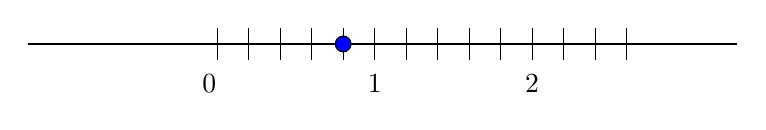
\begin{tikzpicture}
    \draw (-2, 0) -- (7, 0);
    \foreach \x in {0.4, 0.8, ..., 6}
        \draw (\x,-0.2) -- (\x, 0.2);
    
    \draw [fill=blue] (2, 0) circle (0.1);
    \node at (0.3, -0.5) {$0$};
    \node at (2.4, -0.5) {$1$};
    \node at (4.4, -0.5) {$2$};
\end{tikzpicture}
\end{figure}
\begin{choices}
\choice $\frac{1}{5}$
\choice $\frac{2}{5}$ \\
\choice $\frac{3}{4}$ \\
\choice $\frac{4}{5}$ \\
\choice $\frac{5}{6}$ \
\end{choices}
\pause
\begin{tikzpicture}[overlay]
    \node [text = cadmiumgreen] at (1, 1.7) {\cmark};
\end{tikzpicture}
\end{frame}
\begin{frame}
\frametitle{Ejercicio 7}
¿Cuál es el resultado de la operación entre fracciones?
\begin{align*}
\dfrac{1}{3} \cp \dfrac{3}{5} \cp \dfrac{5}{7} \cp \dfrac{7}{9}
\end{align*}
\begin{choices}
\choice $\frac{105}{945}$
\choice $4 \, \frac{12}{35}$ \\
\choice $\frac{345}{567}$ \\
\choice $\frac{100}{165}$ \\
\choice $\frac{945}{10395}$ \
\end{choices}
\pause
\begin{tikzpicture}[overlay]
    \node [text = cadmiumgreen] at (1, 4.3) {\cmark};
\end{tikzpicture}
\end{frame}

\section{Razonamiento visual}
\frame{\tableofcontents[currentsection, hideothersubsections]}
\subsection{Ejercicios}

\begin{frame}
\frametitle{Indicaciones}
En el razonamiento visual, lo que se busca es identificar un patrón que se presenta en la secuencia de figuras.
\\
\bigskip
\pause
Hay que hacer un análisis detallado de la secuencia, para de esa manera elegir la opción correcta.
\end{frame}
\begin{frame}
\frametitle{Ejercicio 8}
¿Qué figura continúa la serie?
\begin{figure}[H]

\begin{tikzpicture}
\draw [thick] (0, 0) rectangle (1, 1);
\draw (0.25, 0.25) rectangle (0.75, 0.75);
\draw (0.25, 0.75) -- (0.5, 0.25); 
\draw (0.5, 0.25) -- (0.7, 0.75);

\draw [thick] (1.5, 0) rectangle (2.5, 1);
\draw [fill] (1.75, 0.25) rectangle (2.25, 0.75);

\draw [thick] (3, 0) rectangle (4, 1);
\draw (3.25, 0.25) rectangle (3.75, 0.75);
\draw (3.25, 0.75) -- (3.5, 0.25); 
\draw (3.5, 0.25) -- (3.75, 0.75);

\draw [thick] (4.5, 0) rectangle (5.5, 1);
\draw [fill] (4.75, 0.25) rectangle (5.25, 0.75);

\draw [dashed, thick] (6, 0) rectangle (7, 1);
\end{tikzpicture}
\end{figure}
\medskip
\begin{figure}[H]
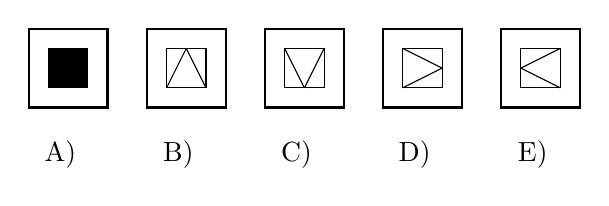
\begin{tikzpicture}
    \draw [thick] (0, 0) rectangle (1, 1);
    \draw [fill] (0.25, 0.25) rectangle (0.75, 0.75);

    \draw [thick] (1.5, 0) rectangle (2.5, 1);
    \draw (1.75, 0.25) rectangle (2.25, 0.75);
    \draw (1.75, 0.25) -- (2, 0.75); 
    \draw (2, 0.75) -- (2.25, 0.25);

    \draw [thick] (3, 0) rectangle (4, 1);
    \draw (3.25, 0.25) rectangle (3.75, 0.75);
    \draw (3.25, 0.75) -- (3.5, 0.25);
    \draw (3.5, 0.25) -- (3.75, 0.75);
   
    \draw [thick] (4.5, 0) rectangle (5.5, 1);
    \draw (4.75, 0.25) rectangle (5.25, 0.75);
    \draw (4.75, 0.75) -- (5.25, 0.5);
    \draw (4.75, 0.25) -- (5.25, 0.5);

    \draw [thick] (6, 0) rectangle (7, 1);
    \draw (6.25, 0.25) rectangle (6.75, 0.75);
    \draw (6.25, 0.5) -- (6.75, 0.75);
    \draw (6.25, 0.5) -- (6.75, 0.25);

    \node at (0.4, -0.6) {A)};
    \node at (1.9, -0.6) {B)};
    \node at (3.4, -0.6) {C)};
    \node at (4.9, -0.6) {D)};
    \node at (6.4, -0.6) {E)};
\end{tikzpicture}
\end{figure}
\pause
\begin{tikzpicture}[overlay]
    \node [text = cadmiumgreen] at (5.3, 0.9) {\cmark};
\end{tikzpicture}
\end{frame}

\begin{frame}
\frametitle{Ejercicio 9}
¿Qué figura continúa la serie?
\medskip
\begin{figure}[H]

\begin{tikzpicture}
    \draw [thick] (0, 0) rectangle (1, 1);
    \draw (0, 0.75) rectangle (0.25, 1);

    \draw [thick] (1.5, 0) rectangle (2.5, 1);
    \draw [fill] (1.5, 0.75) rectangle (1.75, 1);

    \draw [thick] (3, 0) rectangle (4, 1);
    \draw (3, 0.75) rectangle (3.25, 1);
    \draw (3.75, 0.75) rectangle (4, 1);
    
    \draw [thick] (4.5, 0) rectangle (5.5, 1);
    \draw [fill] (4.5, 0.75) rectangle (4.75, 1);
    \draw [fill] (5.25, 0.75) rectangle (5.5, 1);

    \draw [thick, dashed] (6, 0) rectangle (7, 1);
\end{tikzpicture}
\end{figure}
\begin{figure}[H]
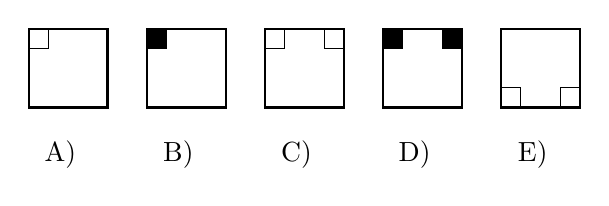
\begin{tikzpicture}
    \draw [thick] (0, 0) rectangle (1, 1);
    \draw (0, 0.75) rectangle (0.25, 1);

    \draw [thick] (1.5, 0) rectangle (2.5, 1);
    \draw [fill] (1.5, 0.75) rectangle (1.75, 1);

    \draw [thick] (3, 0) rectangle (4, 1);
    \draw (3, 0.75) rectangle (3.25, 1);
    \draw (3.75, 0.75) rectangle (4, 1);
    
    \draw [thick] (4.5, 0) rectangle (5.5, 1);
    \draw [fill] (4.5, 0.75) rectangle (4.75, 1);
    \draw [fill] (5.25, 0.75) rectangle (5.5, 1);

    \draw [thick] (6, 0) rectangle (7, 1);
    \draw (6, 0) rectangle (6.25, 0.25);
    \draw (6.75, 0) rectangle (7, 0.25);

    \node at (0.4, -0.6) {A)};
    \node at (1.9, -0.6) {B)};
    \node at (3.4, -0.6) {C)};
    \node at (4.9, -0.6) {D)};
    \node at (6.4, -0.6) {E)};
\end{tikzpicture}
\end{figure}
\pause
\begin{tikzpicture}[overlay]
    \node [text = cadmiumgreen] at (2.3, 0.9) {\cmark};
\end{tikzpicture}
\end{frame}
\begin{frame}
\frametitle{Ejercicio 10}
¿Qué figura continúa la serie?
\medskip
\begin{figure}[H]
    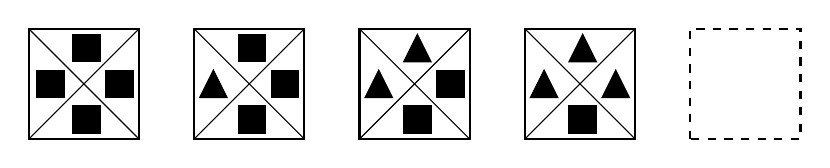
\begin{tikzpicture}[scale=0.7]
    \draw [thick] (0, 0) rectangle (2, 2);
    \draw (0, 0) -- (2, 2);
    \draw (0, 2) -- (2, 0);
    \draw [fill] (0.15, 0.75) rectangle (0.65, 1.25);    
    \draw [fill] (1.4, 0.75) rectangle (1.9, 1.25);    
    \draw [fill] (0.8, 0.1) rectangle (1.3, 0.6);    
    \draw [fill] (0.8, 1.4) rectangle (1.3, 1.9); 
    
    \draw [thick] (3, 0) rectangle (5, 2);
    \draw (3, 2) -- (5, 0);
    \draw (5, 2) -- (3, 0);
    \draw [fill] (3.8, 0.1) rectangle (4.3, 0.6);
    \draw [fill] (3.8, 1.4) rectangle (4.3, 1.9);
    \draw [fill] (4.4, 0.75) rectangle (4.9, 1.25);
    \draw [fill] (3.1, 0.75) -- (3.6, 0.75) -- (3.35, 1.25) -- (3.1, 0.75) -- cycle;

    \draw [thick] (6, 0) rectangle (8, 2);
    \draw (6, 2) -- (8, 0);
    \draw (6, 0) -- (8, 2);
    \draw [fill] (7.4, 0.75) rectangle (7.9, 1.25);
    \draw [fill] (6.8, 0.1) rectangle (7.3, 0.6);
    \draw [fill] (6.1, 0.75) -- (6.6, 0.75) -- (6.35, 1.25) -- (6.1, 0.75) -- cycle;
    \draw [fill] (6.8, 1.4) -- (7.3, 1.4) -- (7.05, 1.9) -- (6.8, 1.4) -- cycle;

    \draw [thick] (9, 0) rectangle (11, 2);
    \draw (9, 2) -- (11, 0);
    \draw (9, 0) -- (11, 2);
    \draw [fill] (9.8, 0.1) rectangle (10.3, 0.6);
    \draw [fill] (9.1, 0.75) -- (9.6, 0.75) -- (9.35, 1.25) -- (9.1, 0.75) -- cycle;
    \draw [fill] (9.8, 1.4) -- (10.3, 1.4) -- (10.05, 1.9) -- (9.8, 1.4) -- cycle;
    \draw [fill] (10.4, 0.75) -- (10.9, 0.75) -- (10.65, 1.25) -- (10.4, 0.75) -- cycle;

    \draw [dashed, thick] (12, 0) rectangle (14, 2);
\end{tikzpicture}
\end{figure}
\begin{figure}[H]
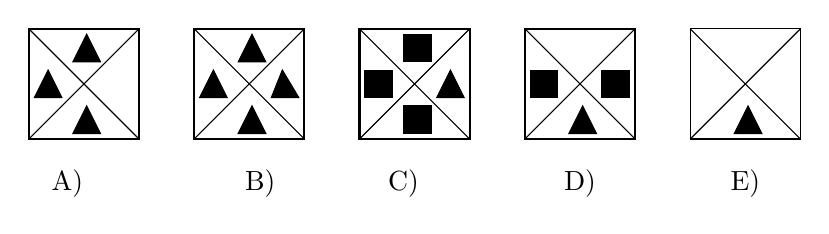
\begin{tikzpicture}[scale=0.7]
    \draw [thick] (0, 0) rectangle (2, 2);
    \draw (0, 2) -- (2, 0);
    \draw (0, 0) -- (2, 2);
    \draw [fill] (0.1, 0.75) -- (0.6, 0.75) -- (0.35, 1.25) -- (0.1, 0.75) -- cycle;
    \draw [fill] (0.8, 0.1) -- (1.3, 0.1) -- (1.05, 0.6) -- (0.8, 0.1) -- cycle;
    \draw [fill] (0.8, 1.4) -- (1.3, 1.4) -- (1.05, 1.9) -- (0.8, 1.4) -- cycle;
   
    \draw [thick] (3, 0) rectangle (5, 2);
    \draw (3, 0) -- (5, 2);
    \draw (3, 2) -- (5, 0);
    \draw [fill] (3.1, 0.75) -- (3.6, 0.75) -- (3.35, 1.25) -- (3.1, 0.75) -- cycle;
    \draw [fill] (3.8, 0.1) -- (4.3, 0.1) -- (4.05, 0.6) -- (3.8, 0.1) -- cycle;
    \draw [fill] (3.8, 1.4) -- (4.3, 1.4) -- (4.05, 1.9) -- (3.8, 1.4) -- cycle;
    \draw [fill] (4.4, 0.75) -- (4.9, 0.75) -- (4.6, 1.25) -- (4.4, 0.75) -- cycle;

    \draw [thick] (6, 0) rectangle (8, 2);
    \draw (6, 2) -- (8, 0);
    \draw (6, 0) -- (8, 2);
    \draw [fill] (6.8, 0.1) rectangle (7.3, 0.6);
    \draw [fill] (6.8, 1.4) rectangle (7.3, 1.9);
    \draw [fill] (6.1, 0.75) rectangle (6.6, 1.25);
    \draw [fill] (7.4, 0.75) -- (7.9, 0.75) -- (7.65, 1.25) -- (7.4, 0.75) -- cycle;

    \draw [thick] (9, 0) rectangle (11, 2);
    \draw (9, 2) -- (11, 0);
    \draw (9, 0) -- (11, 2);
    \draw [fill] (9.1, 0.75) rectangle (9.6, 1.25);
    \draw [fill] (10.4, 0.75) rectangle (10.9, 1.25);
    \draw [fill] (9.8, 0.1) -- (10.3, 0.1) -- (10.05, 0.6) -- (9.8, 0.1) -- cycle;

    \draw (12, 0) rectangle (14, 2);
    \draw (12, 0) -- (14, 2);
    \draw (12, 2) -- (14, 0);
    \draw [fill] (12.8, 0.1) -- (13.3, 0.1) -- (13.05, 0.6) -- (12.8, 0.1) -- cycle;

    \node at (0.7, -0.8) {A)};
    \node at (4.2, -0.8) {B)};
    \node at (6.8, -0.8) {C)};
    \node at (10, -0.8) {D)};
    \node at (13, -0.8) {E)};
    
\end{tikzpicture}
\end{figure}
\pause
\begin{tikzpicture}[overlay]
    \node [text = cadmiumgreen] at (3.4, 0.5) {\cmark};
\end{tikzpicture}
\end{frame}
\begin{frame}
\frametitle{Ejercicio 11}
¿Qué figura continúa en la serie?
\medskip
\begin{figure}[H]

\begin{tikzpicture}[thick]
    \draw (0, 0) rectangle (1,1);
    \draw (0, 0) -- (1, 1);
    \draw (0, 1) -- (1, 0);

    \draw (2, 0) rectangle (3, 1);
    \draw (2, 1) -- (3, 0);

    \draw (4, 0) rectangle (5, 1);

    \draw (6, 1) -- (6, 0) -- (7, 0) -- (7, 1);

    \draw [fill=white, white, text=black] (8, 0) rectangle (9, 1) node [pos=0.5] {$\dots$};
\end{tikzpicture}
\end{figure}
\begin{figure}[h]
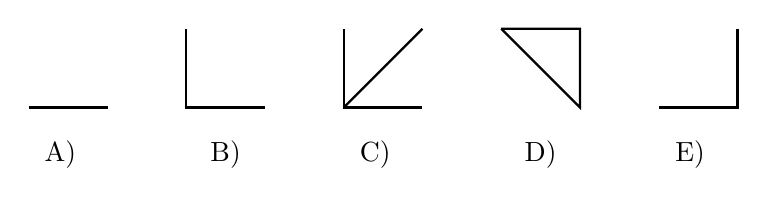
\begin{tikzpicture}[thick]
    \draw (0, 0) -- (1, 0);
    \draw (2, 1) -- (2, 0) -- (3, 0);
    \draw (4, 1) -- (4, 0) -- (5, 0);
    \draw (4, 0) -- (5, 1);
    \draw (6, 1) -- (7, 1) -- (7, 0) -- (6, 1);
    \draw (9, 1) -- (9, 0) -- (8, 0);

    \node at (0.4, -0.6) {A)};
    \node at (2.5, -0.6) {B)};
    \node at (4.4, -0.6) {C)};
    \node at (6.5, -0.6) {D)};
    \node at (8.4, -0.6) {E)};
\end{tikzpicture}
\end{figure}
\pause
\begin{tikzpicture}[overlay]
    \node [text = cadmiumgreen] at (3.5, 0.8) {\cmark};
\end{tikzpicture}
\end{frame}
\begin{frame}
\frametitle{Ejercicio 12}
¿Qué figura continua la serie?
\medskip
\begin{figure}[H]

\begin{tikzpicture}[thick]
    \draw (0, 0) rectangle (1, 1);
    \draw [fill=gray, opacity=0.5] (0, 0) rectangle (0.5, 1);
    
    \draw (2, 0) rectangle (3, 1);
    \draw [fill=gray, opacity=0.5] (2, 0.5) rectangle (3, 1);

    \draw (4, 0) rectangle (5, 1);
    \draw [fill=gray, opacity=0.5] (4.5, 0) rectangle (5, 1);

    \draw (6, 0) rectangle (7, 1);
    \draw [fill=gray, opacity=0.5] (6, 0) rectangle (7, 0.5);

    \draw [fill= white, white, text=black] (8, 0) rectangle (9,1) node [pos=0.5] {$\ldots$};
\end{tikzpicture}
\end{figure}
\begin{figure}[H]
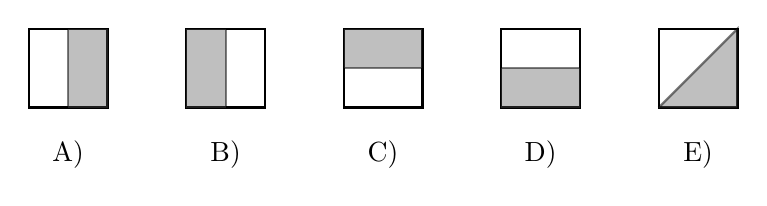
\begin{tikzpicture}[thick]
    \draw (0, 0) rectangle (1, 1);
    \draw [fill=gray, opacity=0.5] (0.5, 0) rectangle (1, 1);
    
    \draw (2, 0) rectangle (3, 1);
    \draw [fill=gray, opacity=0.5] (2, 0) rectangle (2.5, 1);

    \draw (4, 0) rectangle (5, 1);
    \draw [fill=gray, opacity=0.5] (4, 0.5) rectangle (5, 1);

    \draw (6, 0) rectangle (7, 1);
    \draw [fill=gray, opacity=0.5] (6, 0) rectangle (7, 0.5);

    \draw (8, 0) rectangle (9, 1);
    \draw [fill=gray, opacity=0.5] (8, 0) -- (9, 0) -- (9,1) -- (8, 0);

    \node at (0.5, -0.6) {A)};
    \node at (2.5, -0.6) {B)};
    \node at (4.5, -0.6) {C)};
    \node at (6.5, -0.6) {D)};
    \node at (8.5, -0.6) {E)};
\end{tikzpicture}
\end{figure}
\pause
\begin{tikzpicture}[overlay]
    \node [text = cadmiumgreen] at (3.5, 0.8) {\cmark};
\end{tikzpicture}
\end{frame}
\begin{frame}
\frametitle{Ejercicio 13}
¿Cuál de las figuras no guarda relación con las demás?
\medskip
\begin{figure}
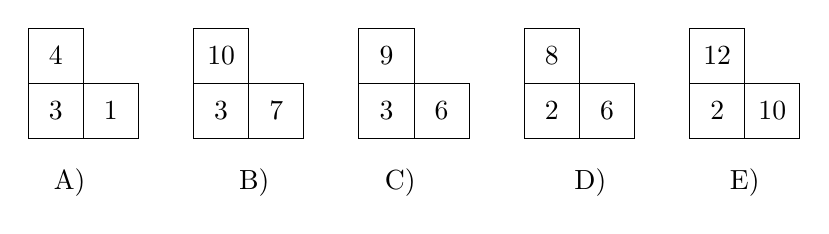
\begin{tikzpicture}[scale=0.7]
    \draw (0, 0) rectangle (1, 1) node [pos=0.5] {$3$};
    \draw (1, 0) rectangle (2, 1) node [pos=0.5] {$1$};
    \draw (0, 1) rectangle (1, 2) node [pos=0.5] {$4$};
    
    \draw (3, 0) rectangle (4, 1) node [pos=0.5] {$3$};
    \draw (4, 0) rectangle (5, 1) node [pos=0.5] {$7$};
    \draw (3, 1) rectangle (4, 2) node [pos=0.5] {$10$};
    
    \draw (6, 0) rectangle (7, 1) node [pos=0.5] {$3$};
    \draw (7, 0) rectangle (8, 1) node [pos=0.5] {$6$};
    \draw (6, 1) rectangle (7, 2) node [pos=0.5] {$9$};
    
    \draw (9, 0) rectangle (10, 1) node [pos=0.5] {$2$};
    \draw (10, 0) rectangle (11, 1) node [pos=0.5] {$6$};
    \draw (9, 1) rectangle (10, 2) node [pos=0.5] {$8$};
    
    \draw (12, 0) rectangle (13, 1) node [pos=0.5] {$2$};
    \draw (13, 0) rectangle (14, 1) node [pos=0.5] {$10$};
    \draw (12, 1) rectangle (13, 2) node [pos=0.5] {$12$};
    
    \node at (0.75, -0.8) {A)};
    \node at (4.1, -0.8) {B)};
    \node at (6.75, -0.8) {C)};
    \node at (10.2, -0.8) {D)};
    \node at (13, -0.8) {E)};
\end{tikzpicture}
\end{figure}
\pause
\begin{tikzpicture}[overlay]
    \node [text = cadmiumgreen] at (5.3, 0.8) {\cmark};
\end{tikzpicture}
\end{frame}
\begin{frame}
\frametitle{Ejercicio 14}
¿Cuál de las siguientes figuras no guarda relación con las demás?
\medskip
\begin{figure}[H]
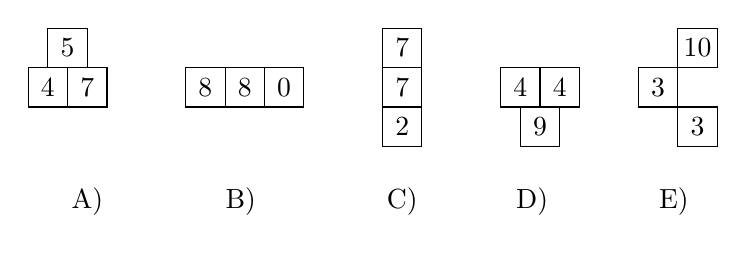
\begin{tikzpicture}
    \draw (0, 0) rectangle (0.5, 0.5) node [pos=0.5] {$4$};
    \draw (0.5, 0) rectangle (1, 0.5) node [pos=0.5] {$7$};
    \draw (0.25, 0.5) rectangle (0.75, 1) node [pos=0.5] {$5$};

    \draw (2, 0) rectangle (2.5, 0.5) node [pos=0.5] {$8$};
    \draw (2.5, 0) rectangle (3, 0.5) node [pos=0.5] {$8$};
    \draw (3, 0) rectangle (3.5, 0.5) node [pos=0.5] {$0$};

    \draw (4.5, 0) rectangle (5, 0.5) node [pos=0.5] {$7$};
    \draw (4.5, 0.5) rectangle (5, 1) node [pos=0.5] {$7$};
    \draw (4.5, 0) rectangle (5, -0.5) node [pos=0.5] {$2$};

    \draw (6, 0) rectangle (6.5, 0.5) node [pos=0.5] {$4$};
    \draw (6.5, 0) rectangle (7, 0.5) node [pos=0.5] {$4$};
    \draw (6.25, 0) rectangle (6.75, -0.5) node [pos=0.5] {$9$};

    \draw (7.75, 0) rectangle (8.25, 0.5)  node [pos=0.5] {$3$};
    \draw (8.25, 0.5) rectangle (8.75, 1)  node [pos=0.5] {$10$};
    \draw (8.25, 0) rectangle (8.75, -0.5)  node [pos=0.5] {$3$};
    
    \node at (0.75, -1.2) {A)};
    \node at (2.7, -1.2) {B)};
    \node at (4.75, -1.2) {C)};
    \node at (6.4, -1.2) {D)};
    \node at (8.2, -1.2) {E)};
\end{tikzpicture}
\end{figure}
\pause
\begin{tikzpicture}[overlay]
    \node [text = cadmiumgreen] at (7.3, 0.8) {\cmark};
\end{tikzpicture}
\end{frame}
\begin{frame}
\frametitle{Ejercicio 15}
Determina una de las raíces de la siguente ecuación de segundo grado:
\begin{align*}
x^{2} - 25 = 0
\end{align*}
\begin{choices}
\choice $-25$
\choice $25$ \\
\choice $5$ \\
\choice $0$ \\
\choice $1.4142$ \
\end{choices}
\pause
\begin{tikzpicture}[overlay]
    \node [text = cadmiumgreen] at (1, 2.5) {\cmark};
\end{tikzpicture}
\end{frame}
\end{document}